\shorthandoff{"}
\chapter{Forschungsergebnisse}
\label{ch:ergebnisse}

\section{Fähigkeiten und Präferenzen der Mitarbeiter}
\label{ch:ergebnisse:analyse}

\subsection{Fähigkeitsbewertungen in Umfrage und Intranet}
\label{ch:ergebnisse:analyse:intranetUndUmfrage}
An der Umfrage unter den Mitarbeitern nahmen $N$=23 Personen aus dem Fachbereich \JES der EXXETA AG teil. Diese Angestellten haben im Rahmen der Befragung 1.408 Präferenzbewertungen abgegeben, welche sich auf 370 einzelne Fähigkeiten verteilen. Das entspricht knapp über 61 abgegebenen Wünschen pro Mitarbeiter. Git ist mit 18 Beurteilungen die meist präferierte Fähigkeit.

Im Intranet des Unternehmens haben die 23 Angestellten 643 Bewertungen hinsichtlich ihrer bereits beherrschten Fähigkeiten abgegeben. Damit verfügt eine Person über etwa 28 Kompetenzen. In Summe beherrschen die Mitarbeiter des Fachbereichs \JES 212 der \anzFaehigkeiten unterschiedlichen, im Intranet gespeicherten Fähigkeiten. Java ist mit 16 Beurteilungen die meist beherrschte Kompetenz.

Abbildung \ref{fig:ergebnisse:analyse:abb1} zeigt, dass sowohl bei Darstellung der präferierten Fähigkeiten als auch bei Betrachtung der beherrschten Kompetenzen der in Kapitel \ref{ch:empfehlungssysteme:cf:speicherbasiert} vorgestellte lange (Ratten-)Schwanz gut erkennbar ist. Dieser ist in beiden Fällen jedoch weniger stark ausgeprägt als in der Referenzdarstellung in Abbildung \ref{fig:empfehlungssysteme:cf:speicherbasiert:abb1}.

\begin{figure}[h]
	\centering
	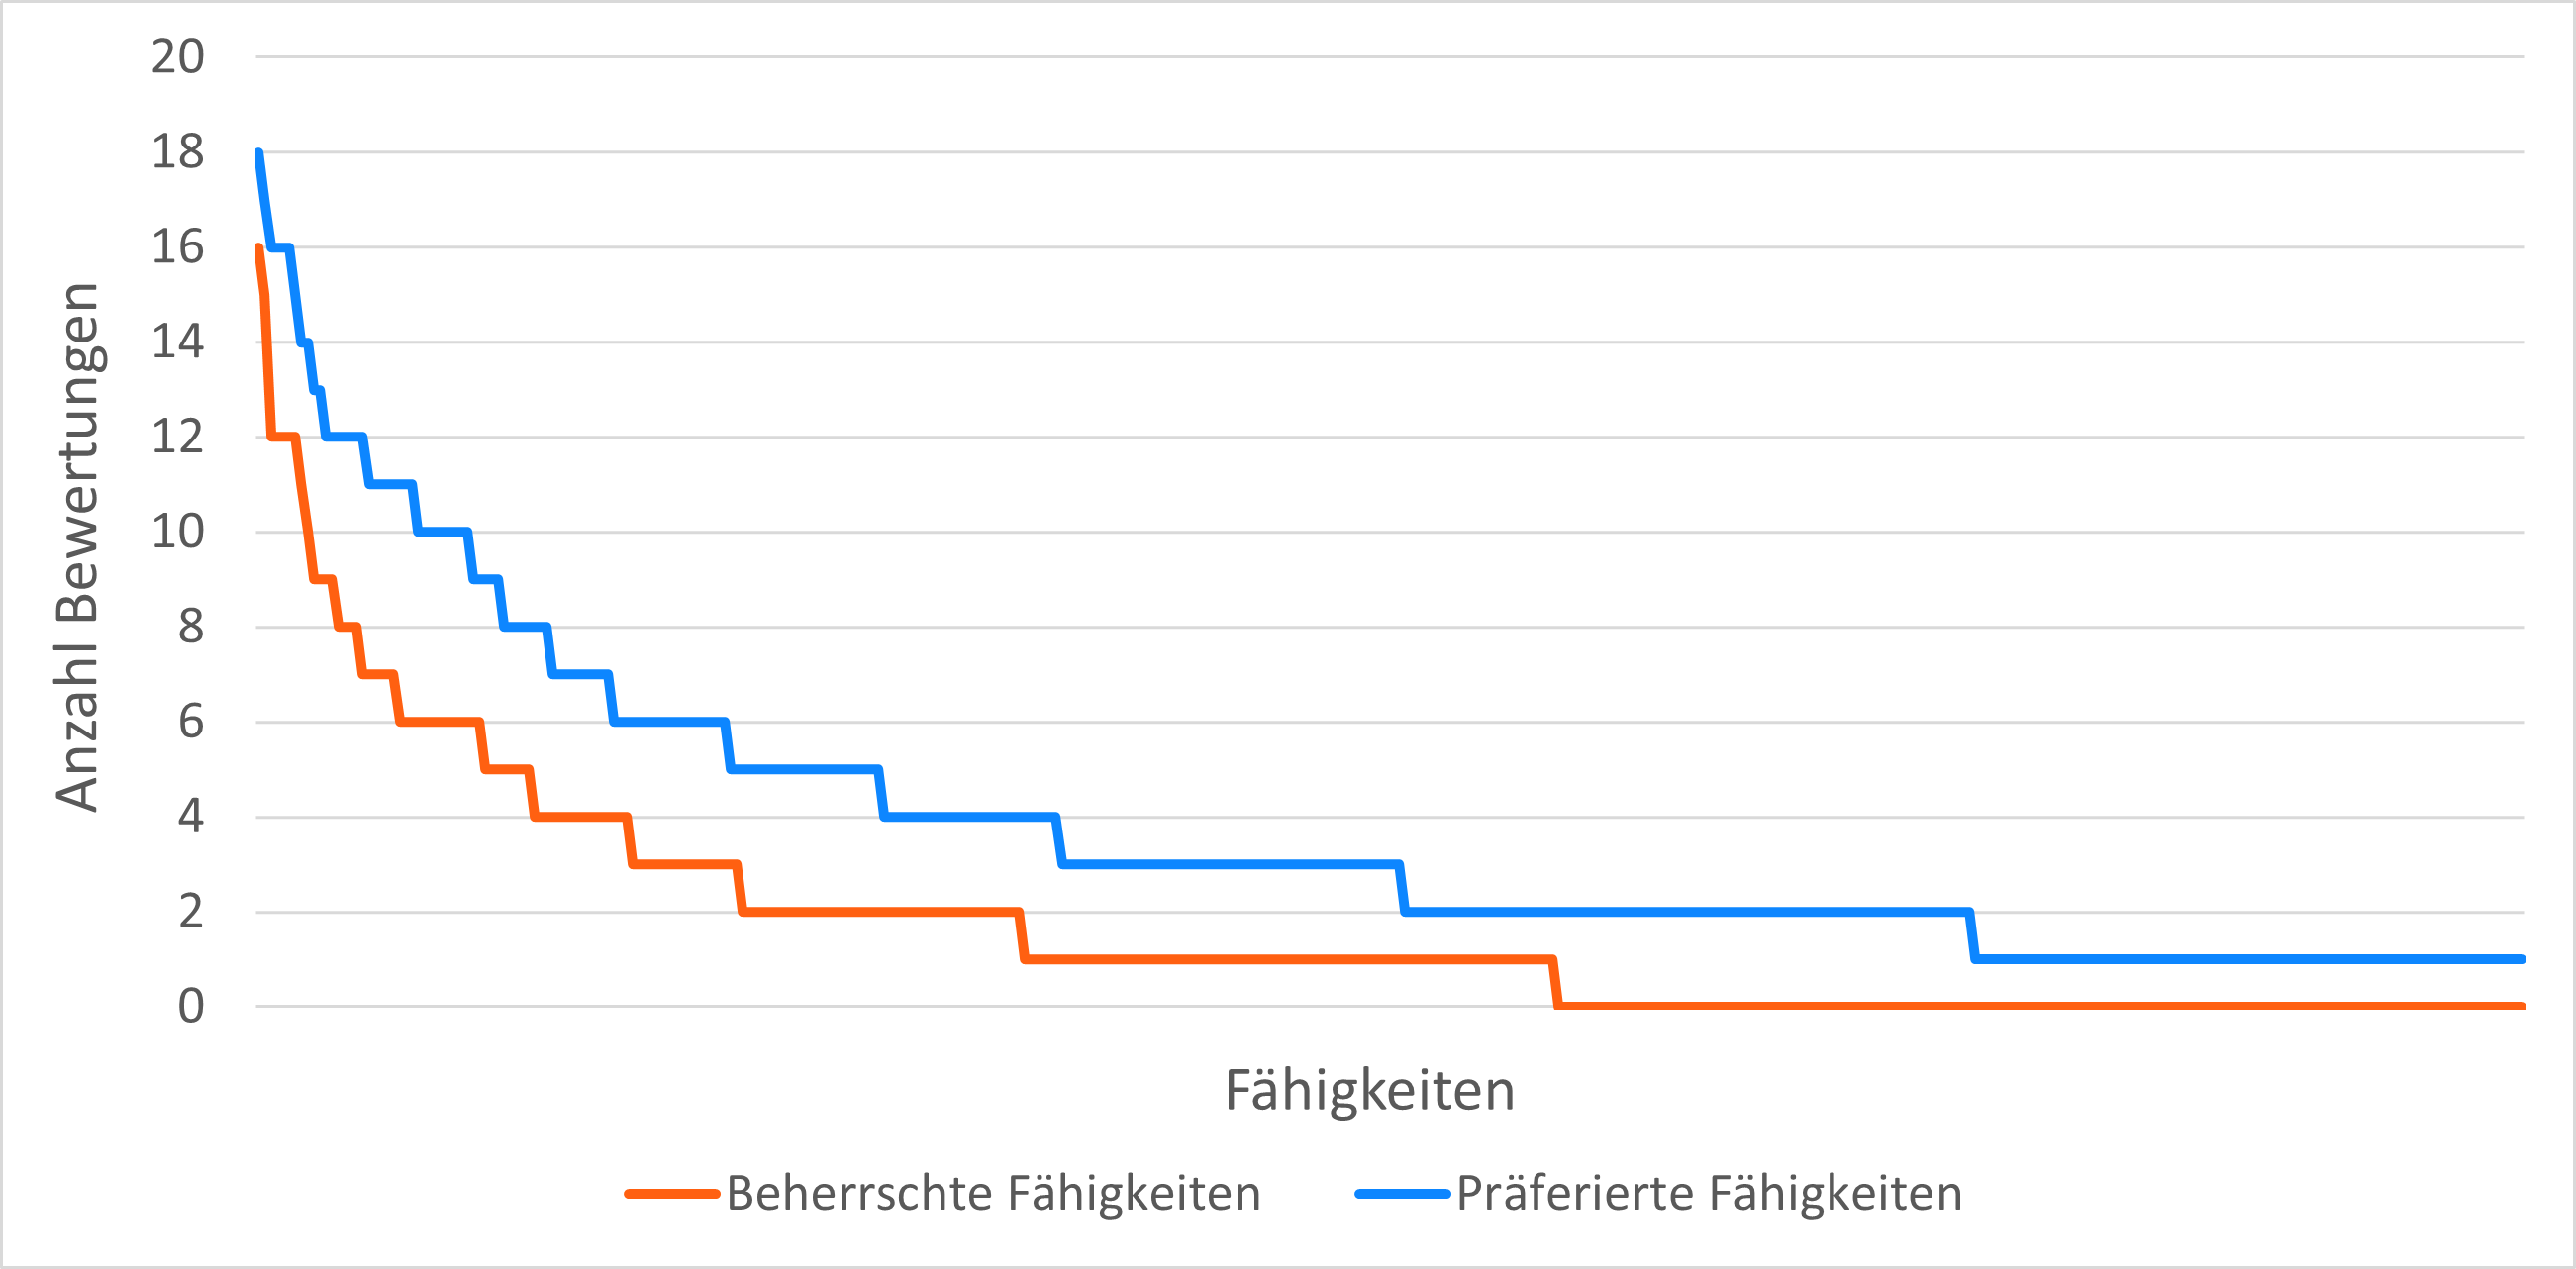
\includegraphics[width=1\textwidth]{gfx/long-tail-insgesamt.png}
	\caption{Langer (Ratten-)Schwanz bei beherrschten und präferierten Fähigkeiten der Mitarbeiter}
	\label{fig:ergebnisse:analyse:abb1}
\end{figure}

Bei der gemeinsamen Betrachtung von Kompetenzen und Wünschen der Mitarbeiter ist festzustellen, dass ein durchschnittlicher Angestellter etwa 75 Fähigkeiten als beherrscht und/oder präferiert bewertet hat. Abbildung \ref{fig:ergebnisse:analyse:abb3} zeigt, zu welchen Anteilen die Kompetenzen als beherrscht und/oder gewünscht markiert wurden.

\begin{figure}[h]
	\centering
	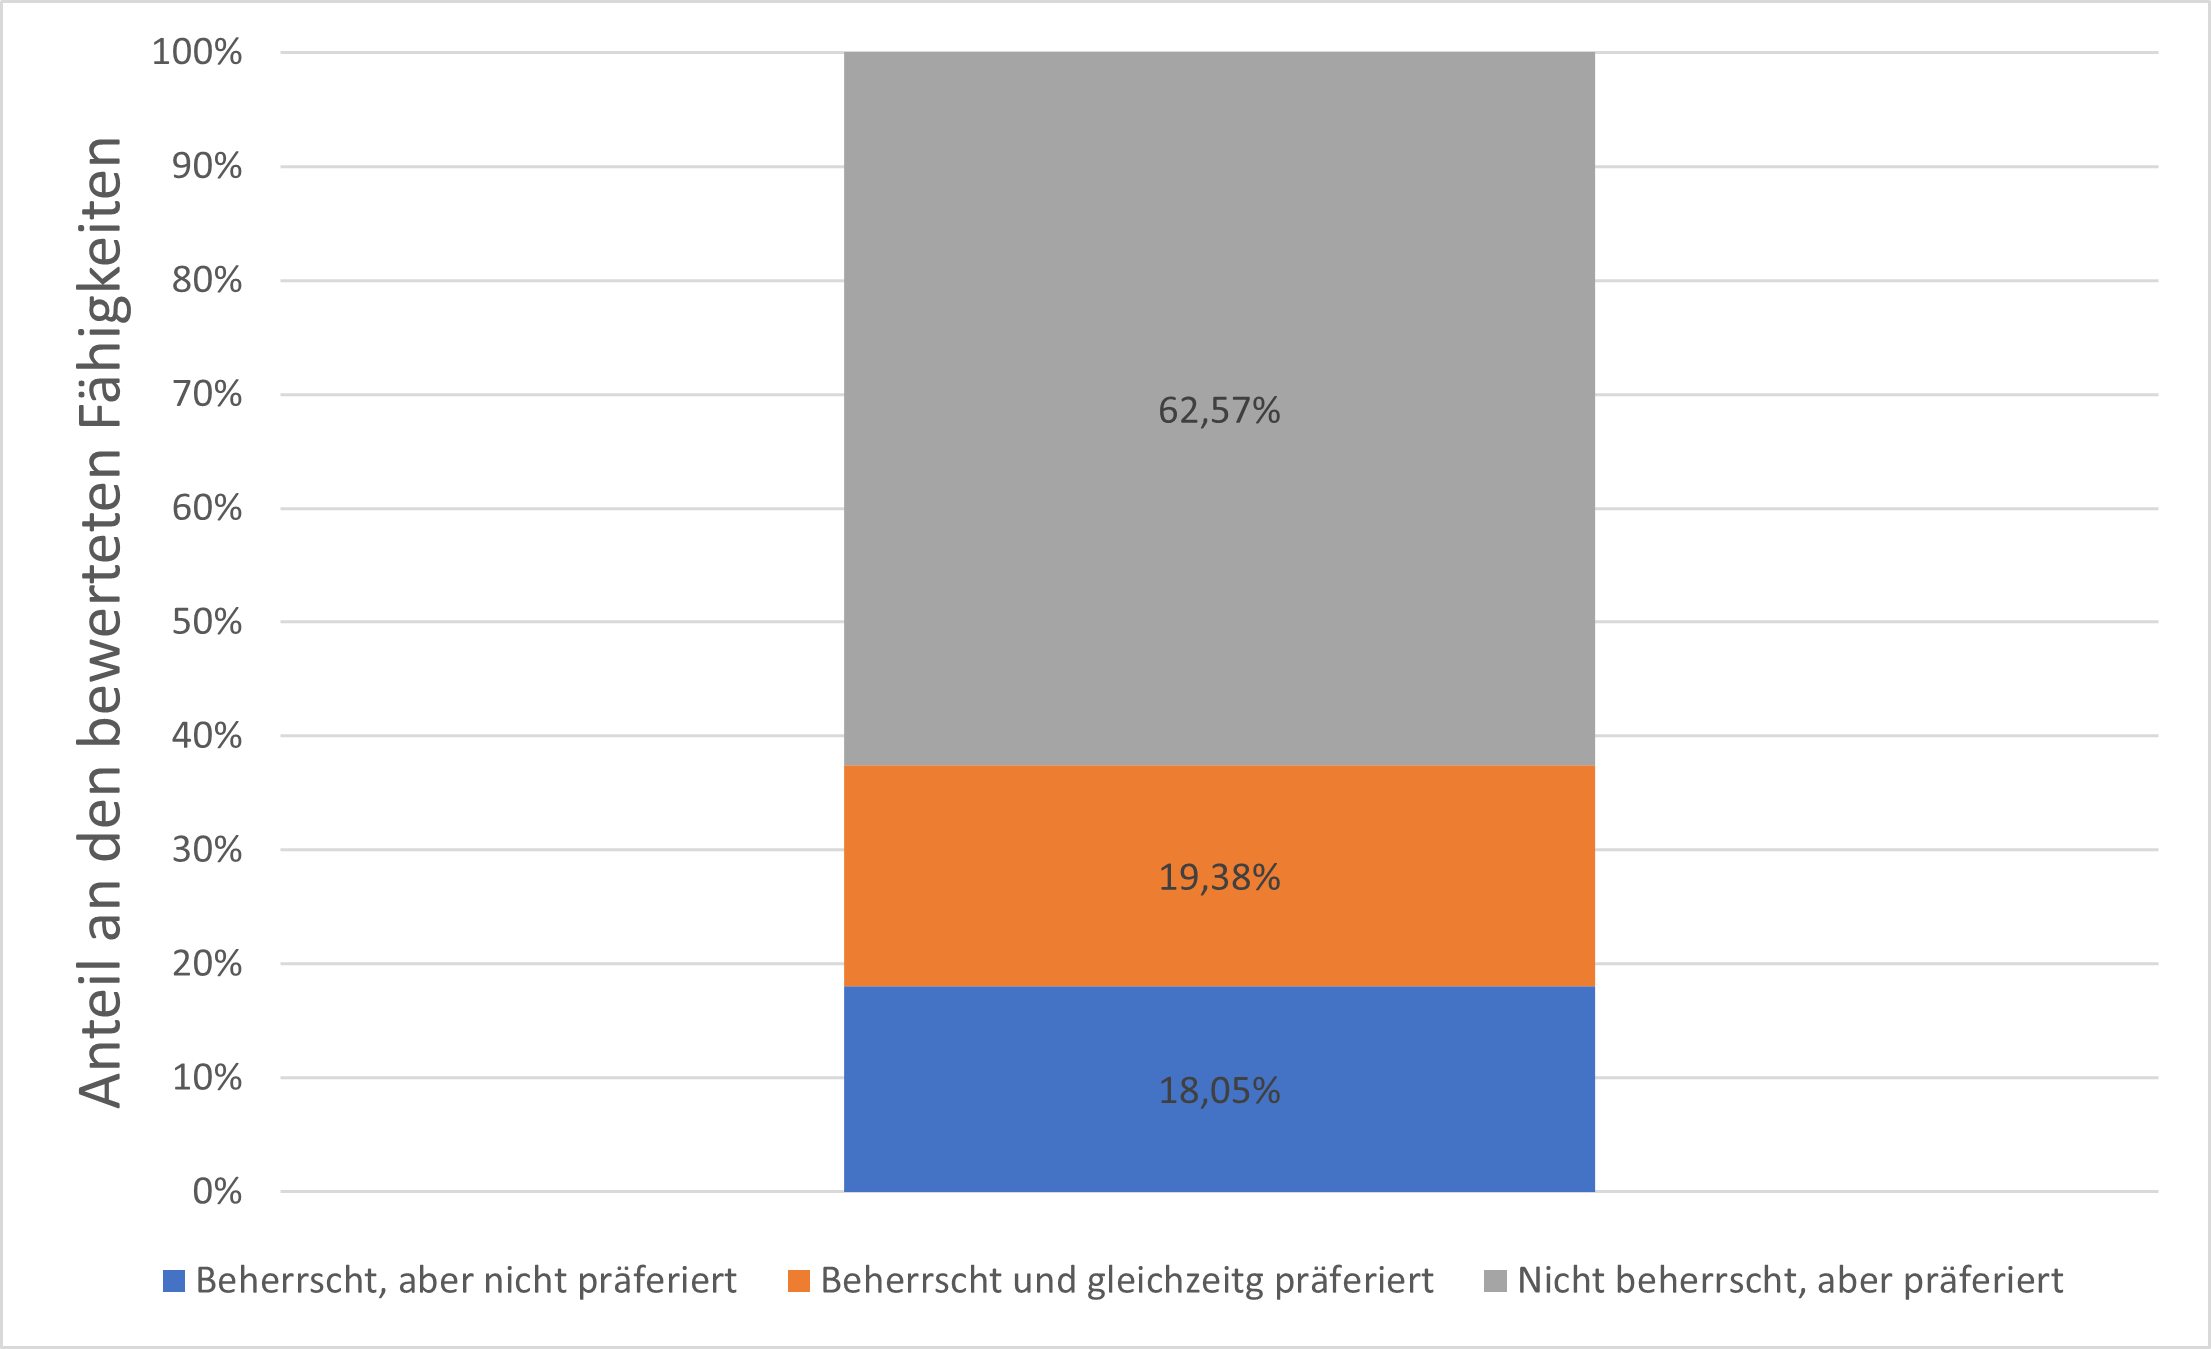
\includegraphics[width=1\textwidth]{gfx/auswertung-anteil-an-faehigkeiten.png}
	\caption{Anteil beherrschter und präferierter Fähigkeiten bei einem durchschnittlichen Mitarbeiter}
	\label{fig:ergebnisse:analyse:abb3}
\end{figure}

In Abbildung \ref{fig:ergebnisse:analyse:abb3} ist zu erkennen, dass ein durchschnittlicher Angestellter ca. 37 Prozent seiner insgesamt beurteilten Kompetenzen gleichzeitig beherrscht (orange markiert und orange-blau schraffiert). Von diesen beherrschten Fähigkeiten werden nur knapp über die Hälfte gewünscht (orange-blau schraffiert). Etwa 63 Prozent aller Fähigkeiten präferiert ein durchschnittlicher Angestellter zwar, beherrscht diese jedoch nicht (blau markiert).

In den vorliegenden Daten des Intranets ist darüber hinaus zu beobachten, dass vier Mitarbeiter keine einzige Fähigkeit bewertet haben. Dies entspricht ca. 17 Prozent der befragten Angestellten. Diese Mitarbeiter sind seit der Einführung des Kompetenz-Bewertungssystems im Intranet durchgehend in einem Projekt tätig und haben daher ihre Fähigkeiten noch nicht gepflegt. Bei der Umfrage bezüglich der Präferenzen gab es keinen Angestellten, welcher keine einzige Fähigkeit als Wunsch ausgewählte.
\newpage
\subsection{Bewertungen hinsichtlich der Projektpositionen}
\label{ch:ergebnisse:analyse:projektpositionen}
Im Rahmen der vorliegenden Master-Thesis wurden fünf beispielhafte Projektpositionen definiert und in Kapitel \ref{ch:methodik:evaluation} vorgestellt. Abbildung \ref{fig:ergebnisse:analyse:abb5} zeigt, welcher Anteil an befragten Mitarbeitern die durchschnittlich gesuchte Fähigkeit jeder Stelle beherrscht bzw. präferiert.

\begin{figure}[h]
	\centering
	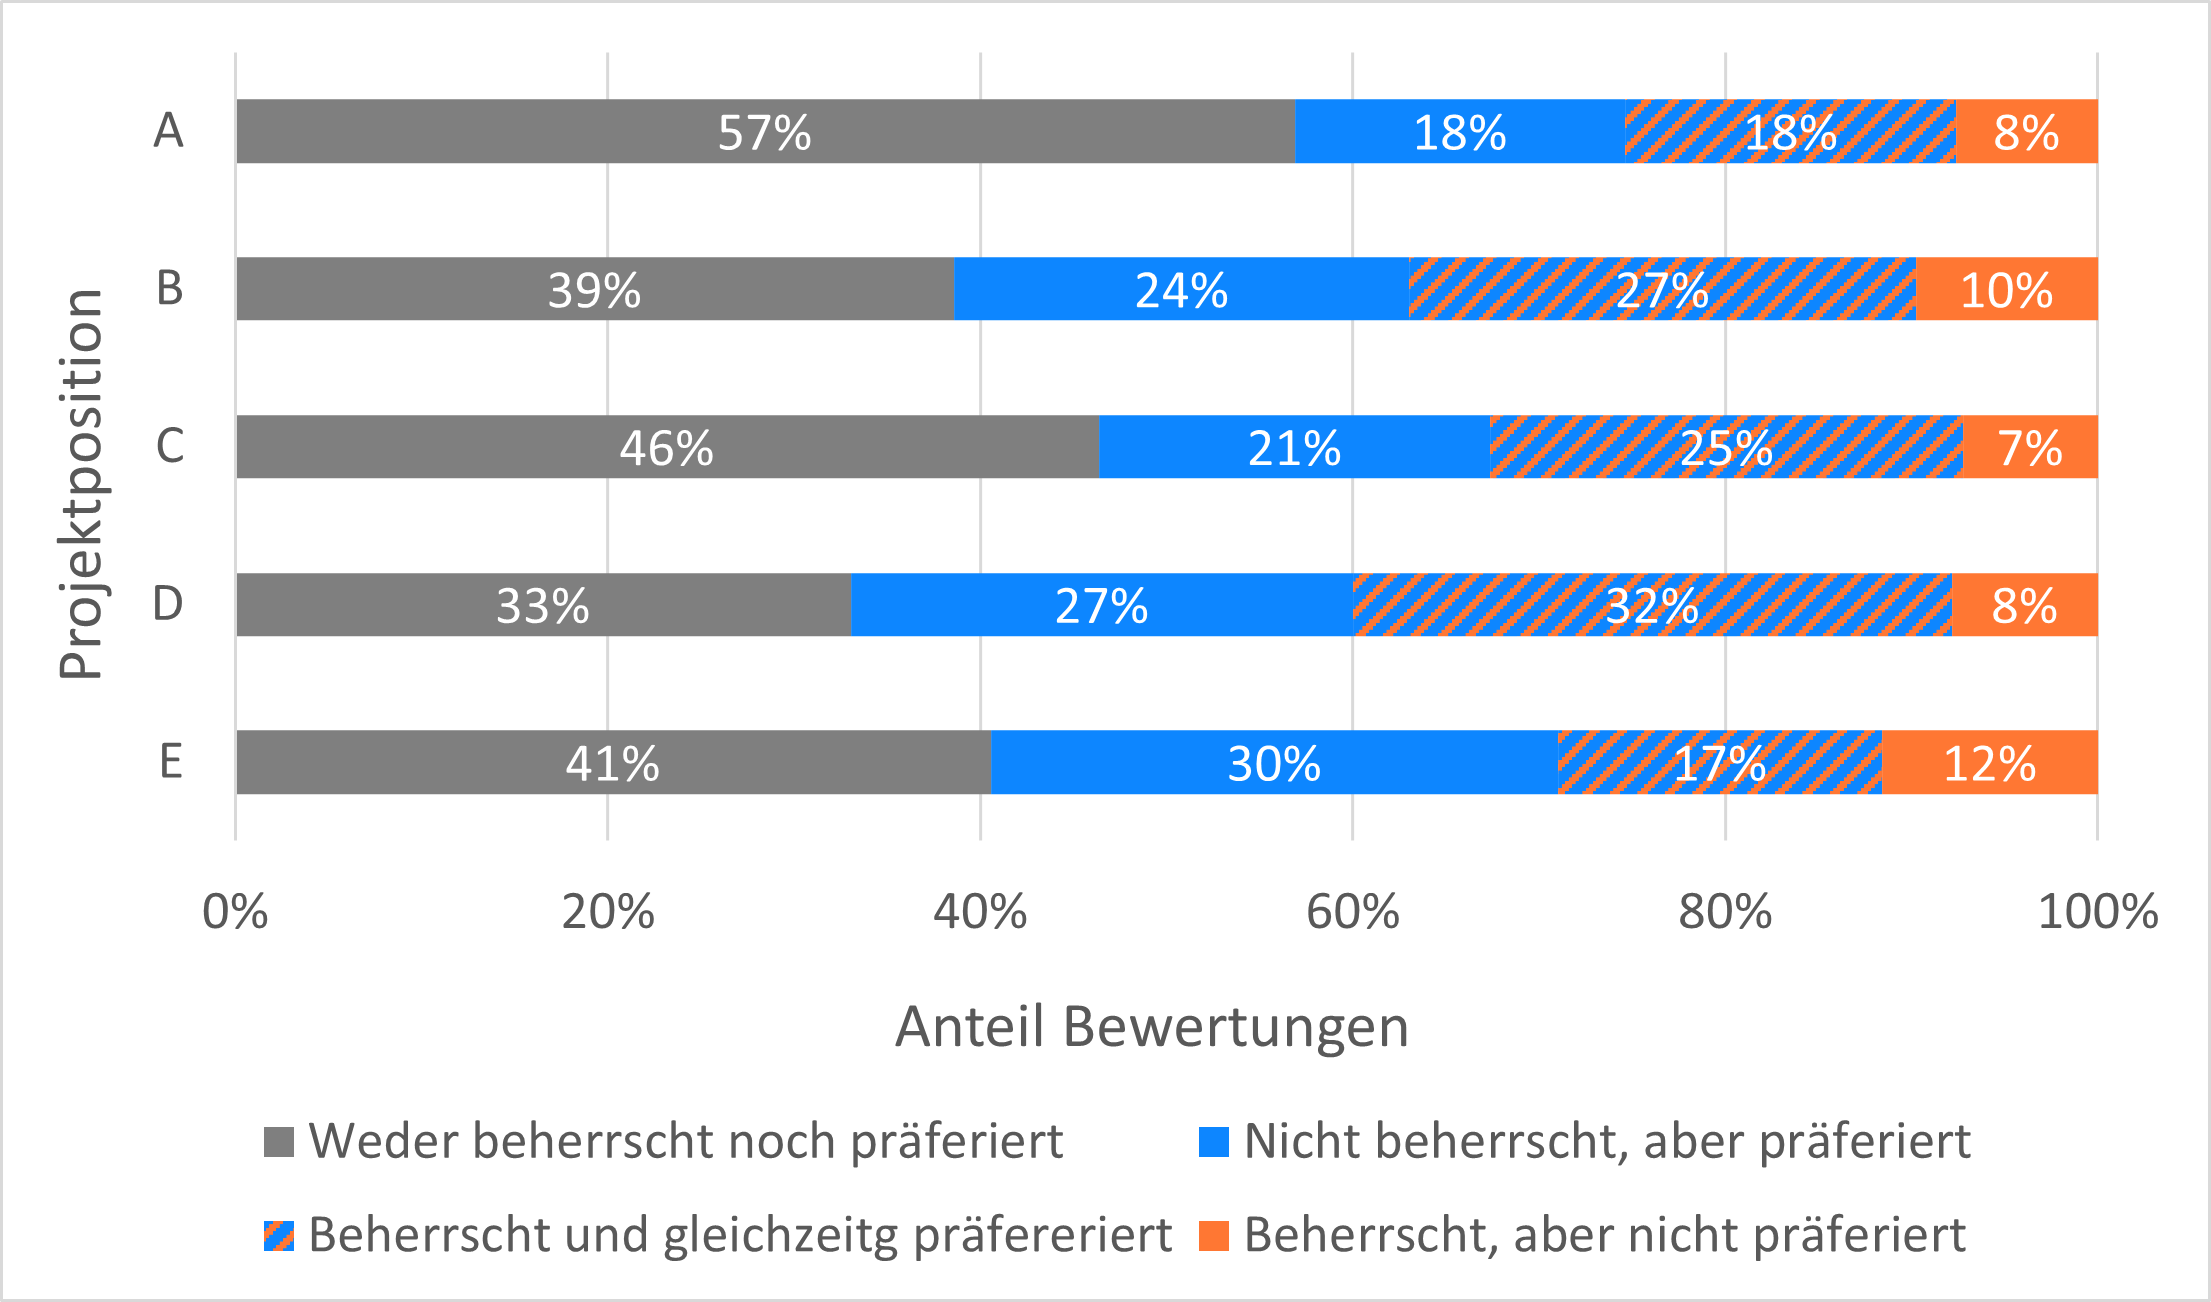
\includegraphics[width=1\textwidth]{gfx/anteil-bewertungen-je-projektposition.png}
	\caption{Anteile an Mitarbeitern, welche die in den Beispielprojektpositionen gesuchten Fähigkeiten beherrschen und/oder präferieren}
	\label{fig:ergebnisse:analyse:abb5}
\end{figure}

In Abbildung \ref{fig:ergebnisse:analyse:abb5} ist zu erkennen, dass ca. ein Drittel der befragten Mitarbeiter die durchschnittlich gesuchte Fähigkeit jeder Projektposition beherrschen (orange markiert und orange-blau schraffiert). Außerdem präferieren etwa 28 Prozent der Angestellten, welche über eine gesuchte Fähigkeit verfügen (orange markiert und orange-blau schraffiert), deren Anwendung nicht (orange markiert). Abschließend ist in Abbildung \ref{fig:ergebnisse:analyse:abb5} zu beobachten, dass die orange-blau schraffierten und blau markierten Anteile an Mitarbeitern im Durchschnitt gleich groß sind.

\newpage
\section{Ergebnisse der Fallstudie}
\label{ch:ergebnisse:fallstudie}

\subsection{Erwartete Zufriedenheit der Mitarbeiter}
\label{ch:ergebnisse:fallstudie:umfrageMitarbeiter}
In der Umfrage unter den 23 Angestellten der EXXETA AG wurde erhoben, welche Zufriedenheit diese mit Tätigkeiten auf den fünf vordefinierten Projektpositionen prognostizieren. Die Ergebnisse sind in Abbildung \ref{fig:ergebnisse:fallstudie:abb1} dargestellt.

\begin{figure}[h]
	\centering
	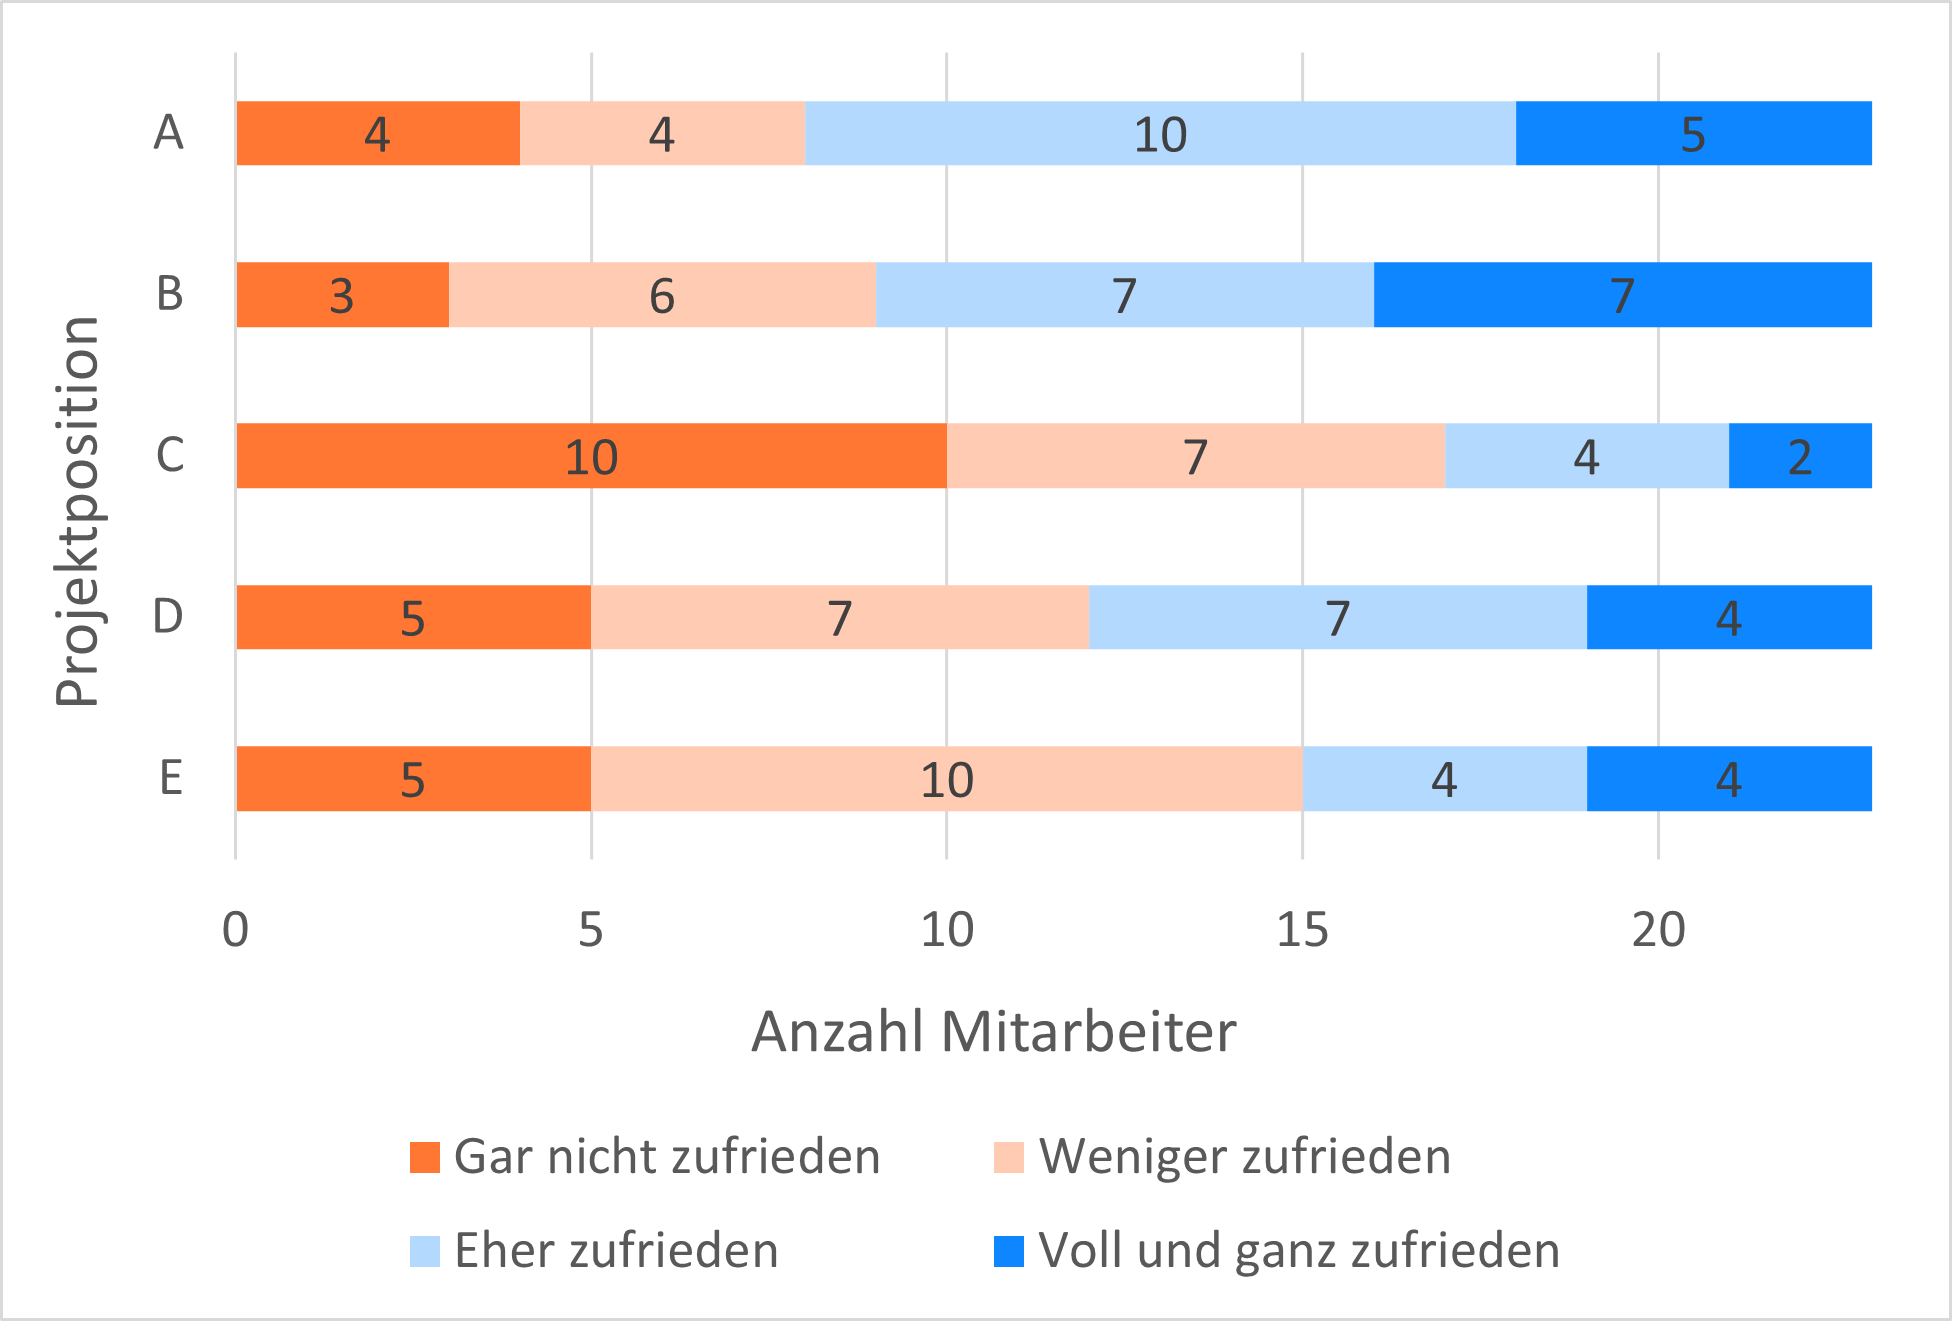
\includegraphics[width=1\textwidth]{gfx/mitarbeiter-zufriedenheit-umfrage.png}
	\caption{Anzahl an Mitarbeitern, welche zufrieden bzw. unzufrieden mit der Tätigkeit auf den jeweiligen vordefinierten Projektpositionen wären}
	\label{fig:ergebnisse:fallstudie:abb1}
\end{figure}

In Abbildung \ref{fig:ergebnisse:fallstudie:abb1} ist zu erkennen, dass sich die Mitarbeiter überwiegend zufrieden mit den Projektpositionen A und B zeigen. Tätigkeiten auf den Stellen C und E lehnen die Angestellten dagegen überwiegend ab. Projektposition D stehen die Mitarbeiter gespalten gegenüber, sodass etwa die Hälfte der Befragten zufrieden und die andere Hälfte unzufrieden mit dieser Tätigkeit ist.
\newpage
\subsection{Positionierung der Mitarbeiter}
\label{ch:ergebnisse:fallstudie:positionierungMitarbeiter}
Abbildung \ref{fig:ergebnisse:analyse:abb7} zeigt, für wie viele der 23 befragten Mitarbeiter der bilaterale Empfehlungsansatz gegenüber dem unilateralen Vorgehen für eine höhere Zufriedenheit seitens der Angestellten sorgte. Wie in Kapitel \ref{ch:methodik:evaluation} beschrieben, wird die Entstehung eines höheren Wohlbefindens angenommen, wenn das bilaterale System die Angestellten bei einer prognostizierten Zufriedenheit höher und bei einer erwarteten Unzufriedenheit niedriger positioniert als die unilaterale Anwendung.

\begin{figure}[h]
	\centering
	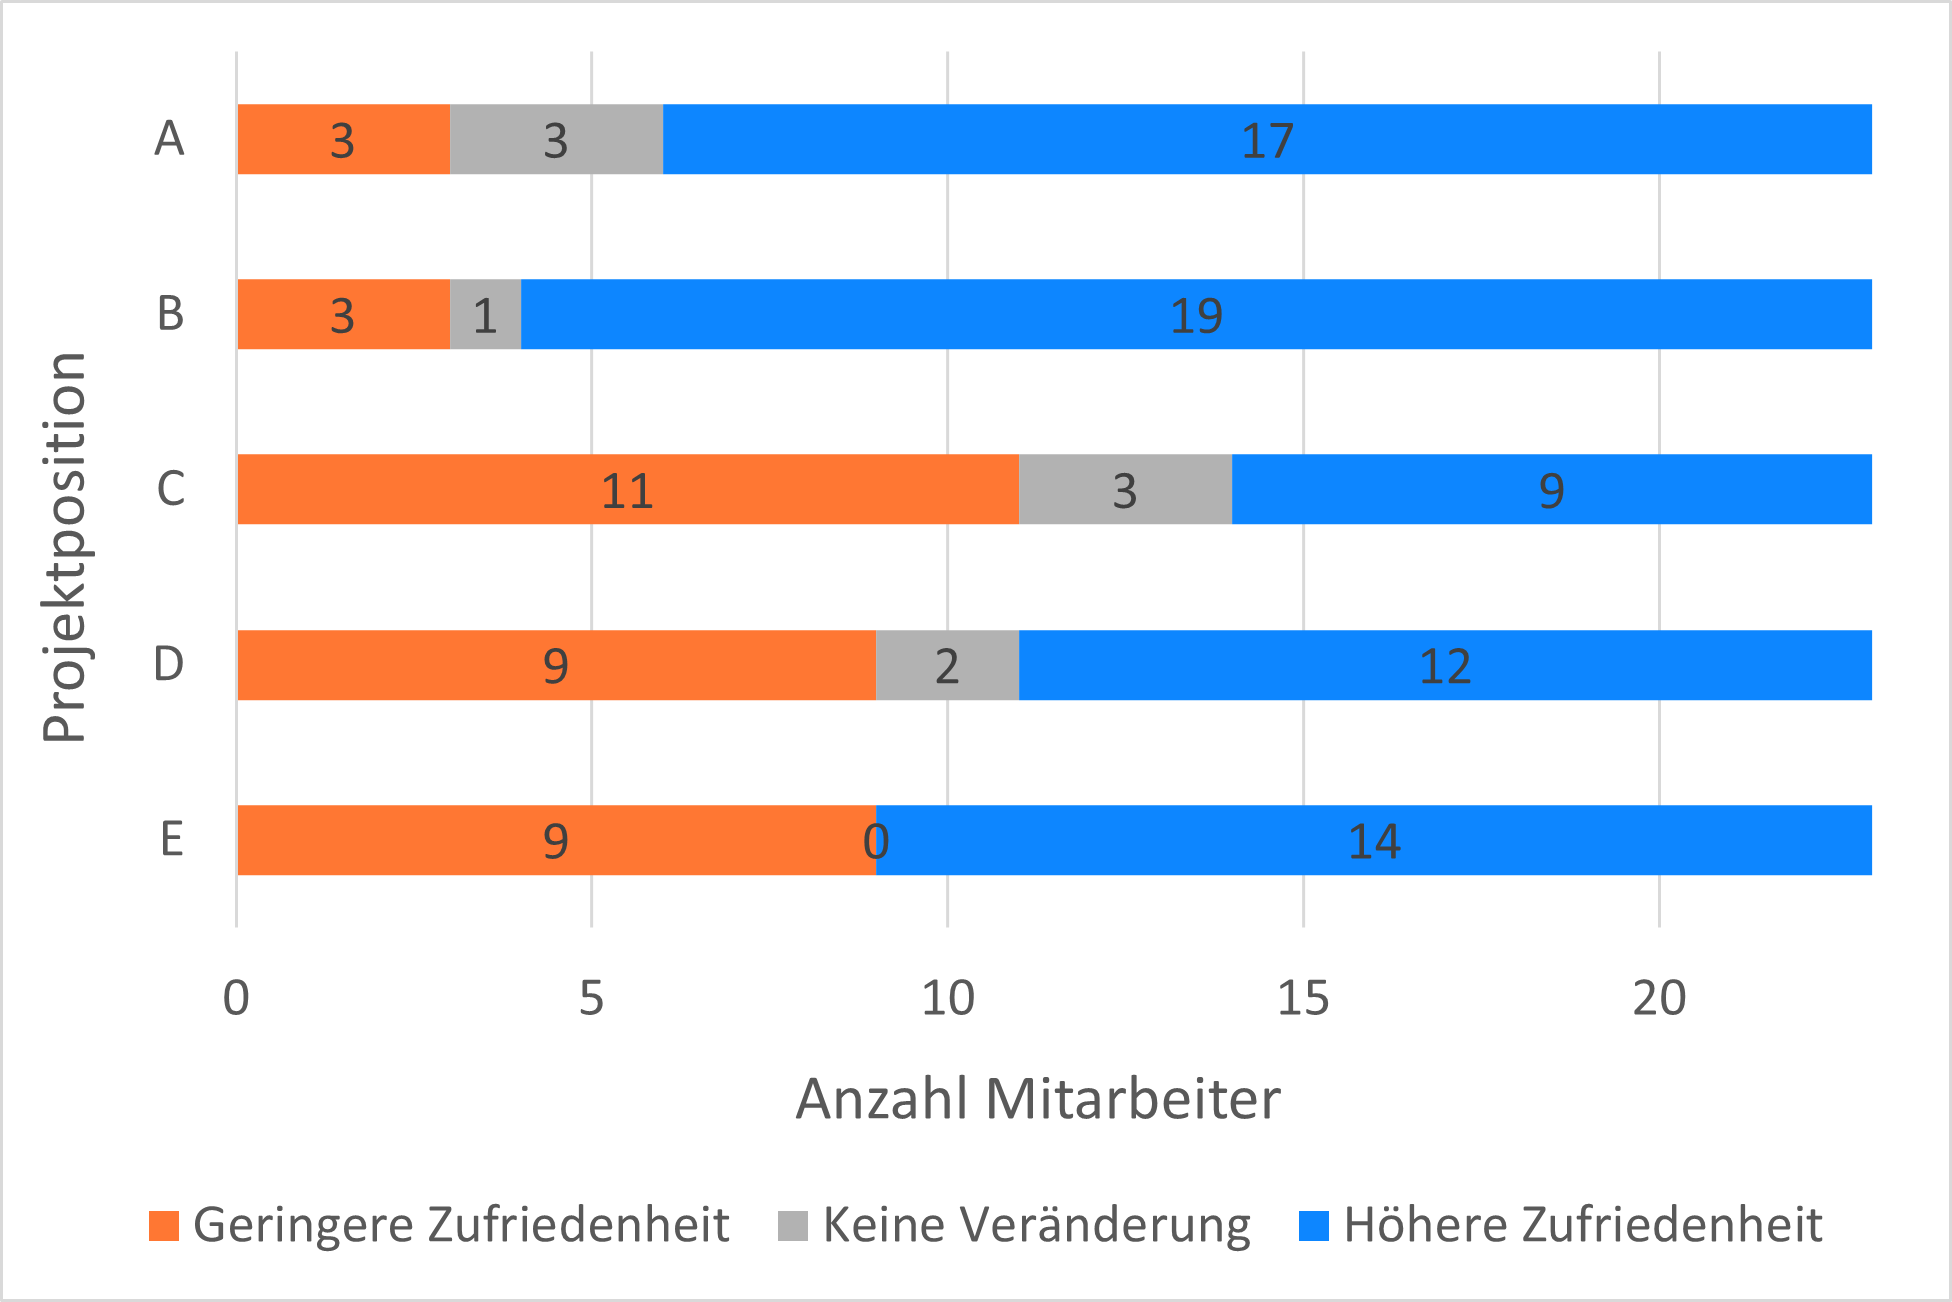
\includegraphics[width=1\textwidth]{gfx/zufriedenheit-projekte.png}	
	\caption{Ergebnisse des bilateralen Empfehlungsansatzes im Vergleich zum unilateralen Vorgehen hinsichtlich der Mitarbeiterzufriedenheit}
	\label{fig:ergebnisse:analyse:abb7}
\end{figure}
In Abbildung \ref{fig:ergebnisse:analyse:abb7} ist zu erkennen, dass der bilaterale Empfehlungsansatz einen Großteil der Angestellten für die Projektpositionen A und B zugunsten einer höheren Zufriedenheit positionierte. Bei den Projektpositionen D und E erreichte das bilaterale Vorschlagsverfahren für knapp über die Hälfte der Mitarbeiter eine höhere Zufriedenheit. Lediglich bei Projektposition C erzielte der bilaterale Empfehlungsansatz im Vergleich zur unilateralen Variante eine geringere Zufriedenheit.
\newpage
\subsection{Prognostizierte Arbeitsleistung der Projektmanager}
\label{ch:ergebnisse:fallstudie:arbeitsleistung}
An der Umfrage unter den Projektmanagern nahmen $N$=7 Personen teil. Sechs Befragte sind im Bereich \JES tätig. Ein Teilnehmer stammt aus einer anderen Abteilung, welche jedoch ähnliche Technologien bei der Projekttätigkeit einsetzt. Abbildung \ref{fig:ergebnisse:fallstudie:arbeitsleistung:abb1} zeigt, von den vorgeschlagenen Mitarbeitern welches Empfehlungsansatzes die Projektmanager eine höhere Arbeitsleistung erwarten.

\begin{figure}[h]
	\centering
	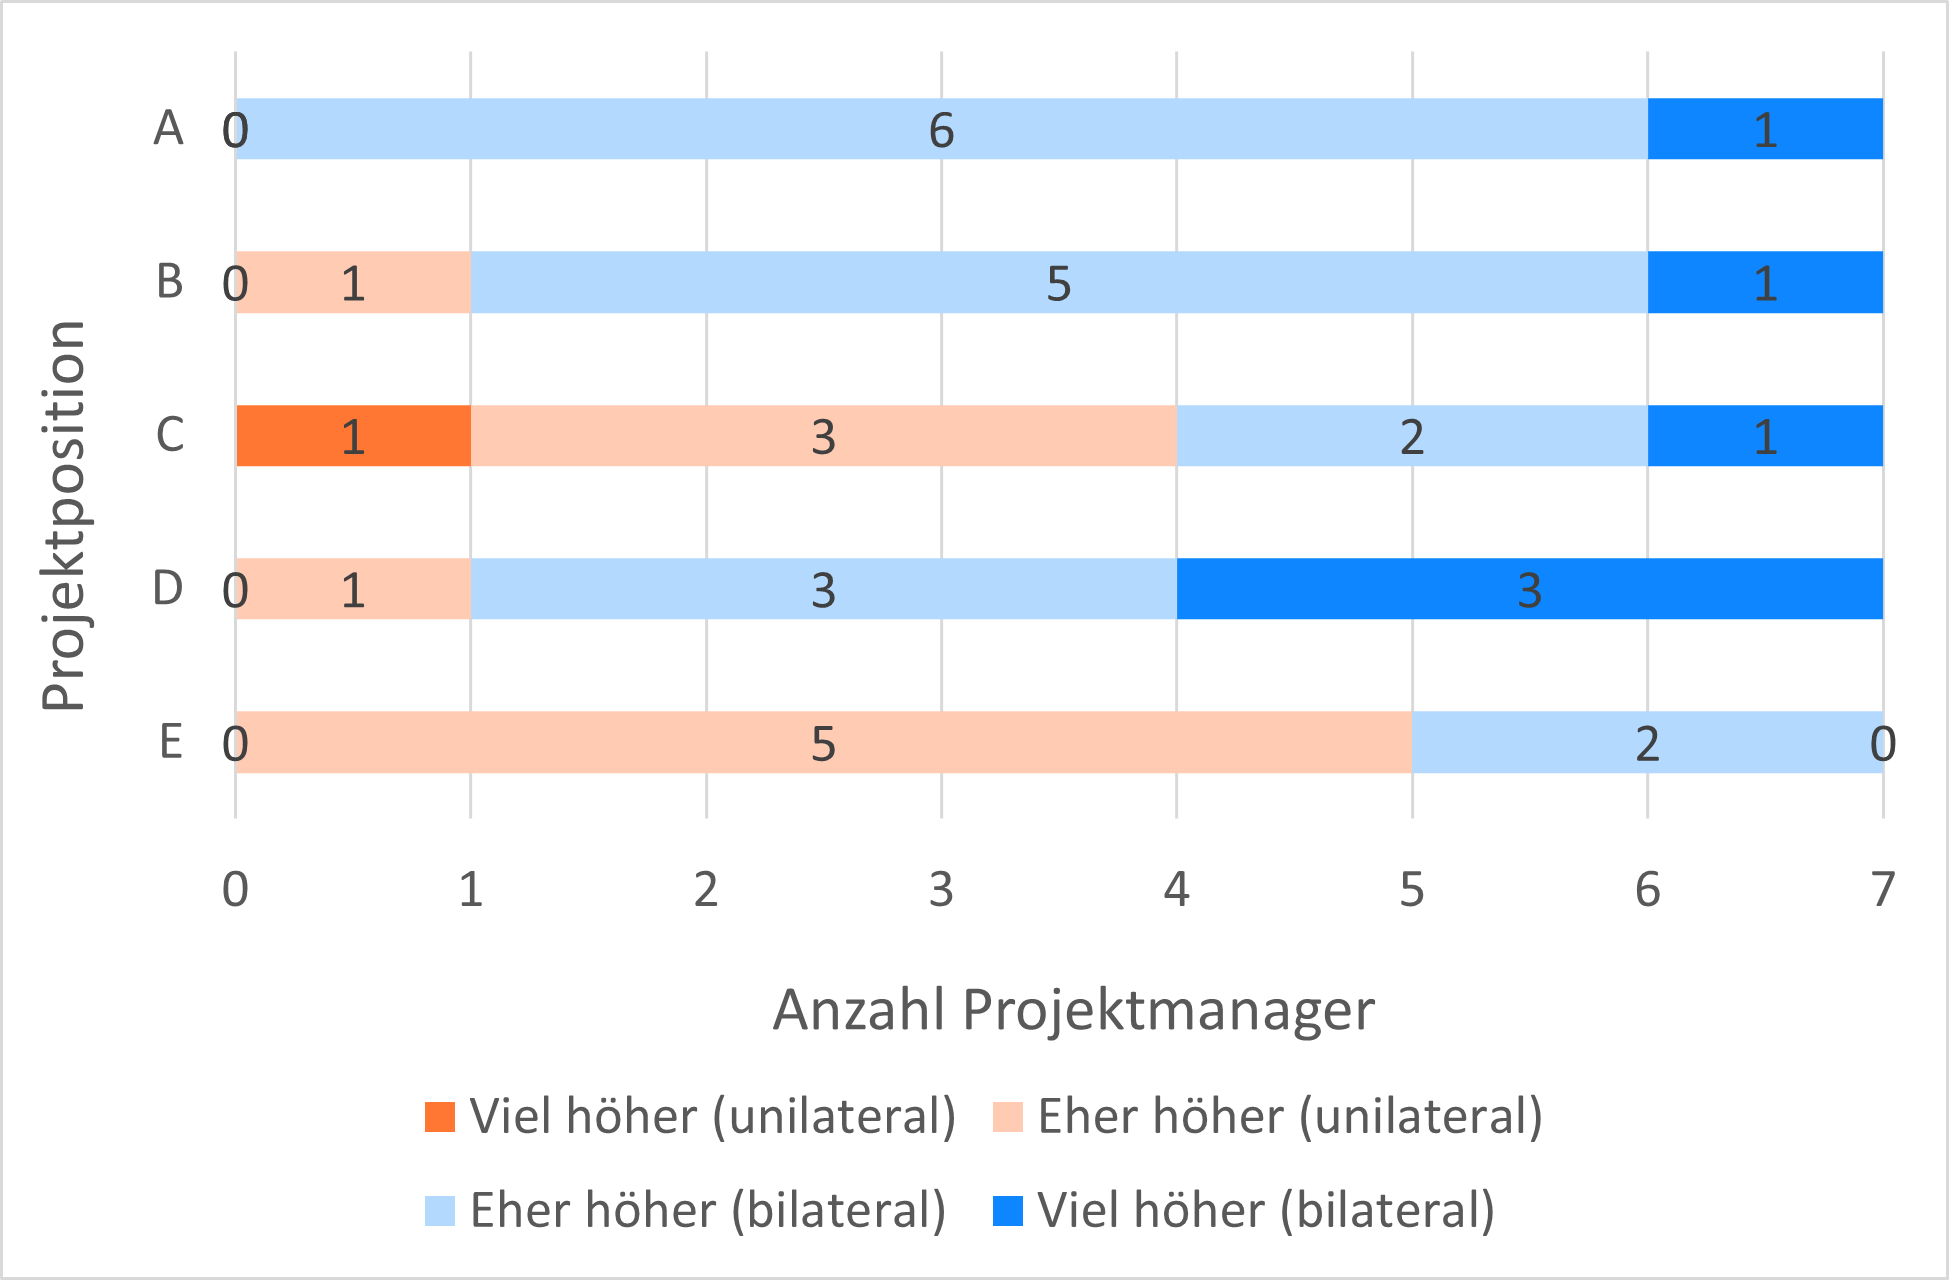
\includegraphics[width=1\textwidth]{gfx/ergebnisse-projektmanager-arbeitsleistung.png}	
	\caption{Ergebnisse der Umfrage unter den Projektmanager hinsichtlich der erwarteten Arbeitsleistung der Mitarbeiter}
	\label{fig:ergebnisse:fallstudie:arbeitsleistung:abb1}
\end{figure}

An den Ergebnissen in Abbildung \ref{fig:ergebnisse:fallstudie:arbeitsleistung:abb1} ist zu erkennen, dass die Projektmanager bei drei der fünf vordefinierten Projektpositionen von den vorgeschlagenen Mitarbeitern des bilateralen Empfehlungsansatzes eine höhere Arbeitsleistung erwarten. Bei Projektposition A geht sogar kein einziger Projektmanager von einer höhere Leistung von den Empfehlungen des unilateralen Verfahrens aus. Auffällig ist außerdem, dass die Hälfte der Teilnehmer von den Vorschlägen des bilateralen Empfehlungssystems für Projektposition D eine viel höhere Arbeitsleistung prognostizieren. Bei den Empfehlungen für die Projektpositionen C und E bewerten die Projektmanager jedoch die Arbeitsleistungen des unilateralen Empfehlungsansatzes gegenüber der bilateralen Variante als höher.
\newpage
\subsection{Einschätzungen hinsichtlich möglicher Unterforderung}
\label{ch:ergebnisse:fallstudie:kurven}
Sowohl unter den Projektmanagern als auch den Mitarbeitern wurde in den jeweiligen Umfragen erhoben, wie sie mögliche Unterforderung bei der Projektarbeit bewerten. Die Ergebnisse sind in Abbildung \ref{fig:ergebnisse:fallstudie:kurven:abb1} dargestellt. In der Grafik wurden die Antwortmöglichkeiten der Umfragen durch die entsprechenden Kurven aus Darstellung \ref{fig:methodik:versuchsaufbau:unilateral:abb2} ersetzt.

\begin{figure}[h]
	\centering
	
	\subfloat[Projektmanager]{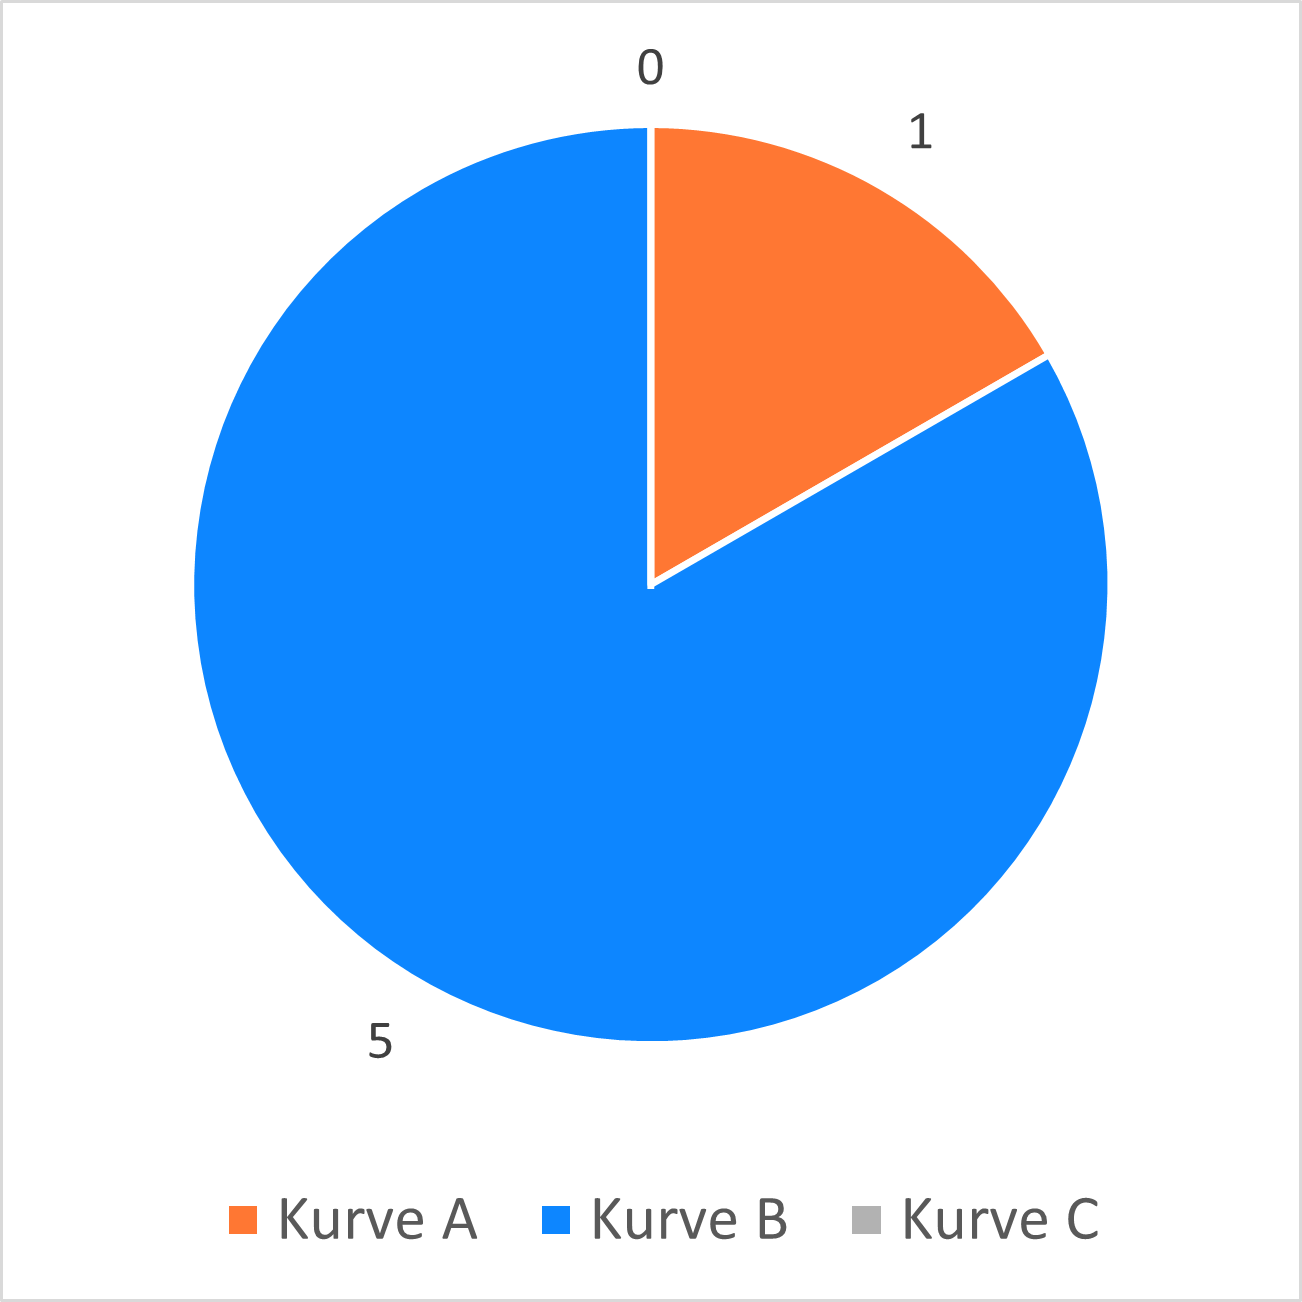
\includegraphics[width = 0.5\textwidth]{gfx/ergebis-kurve-projektmanager.png}}
	\subfloat[Mitarbeiter]{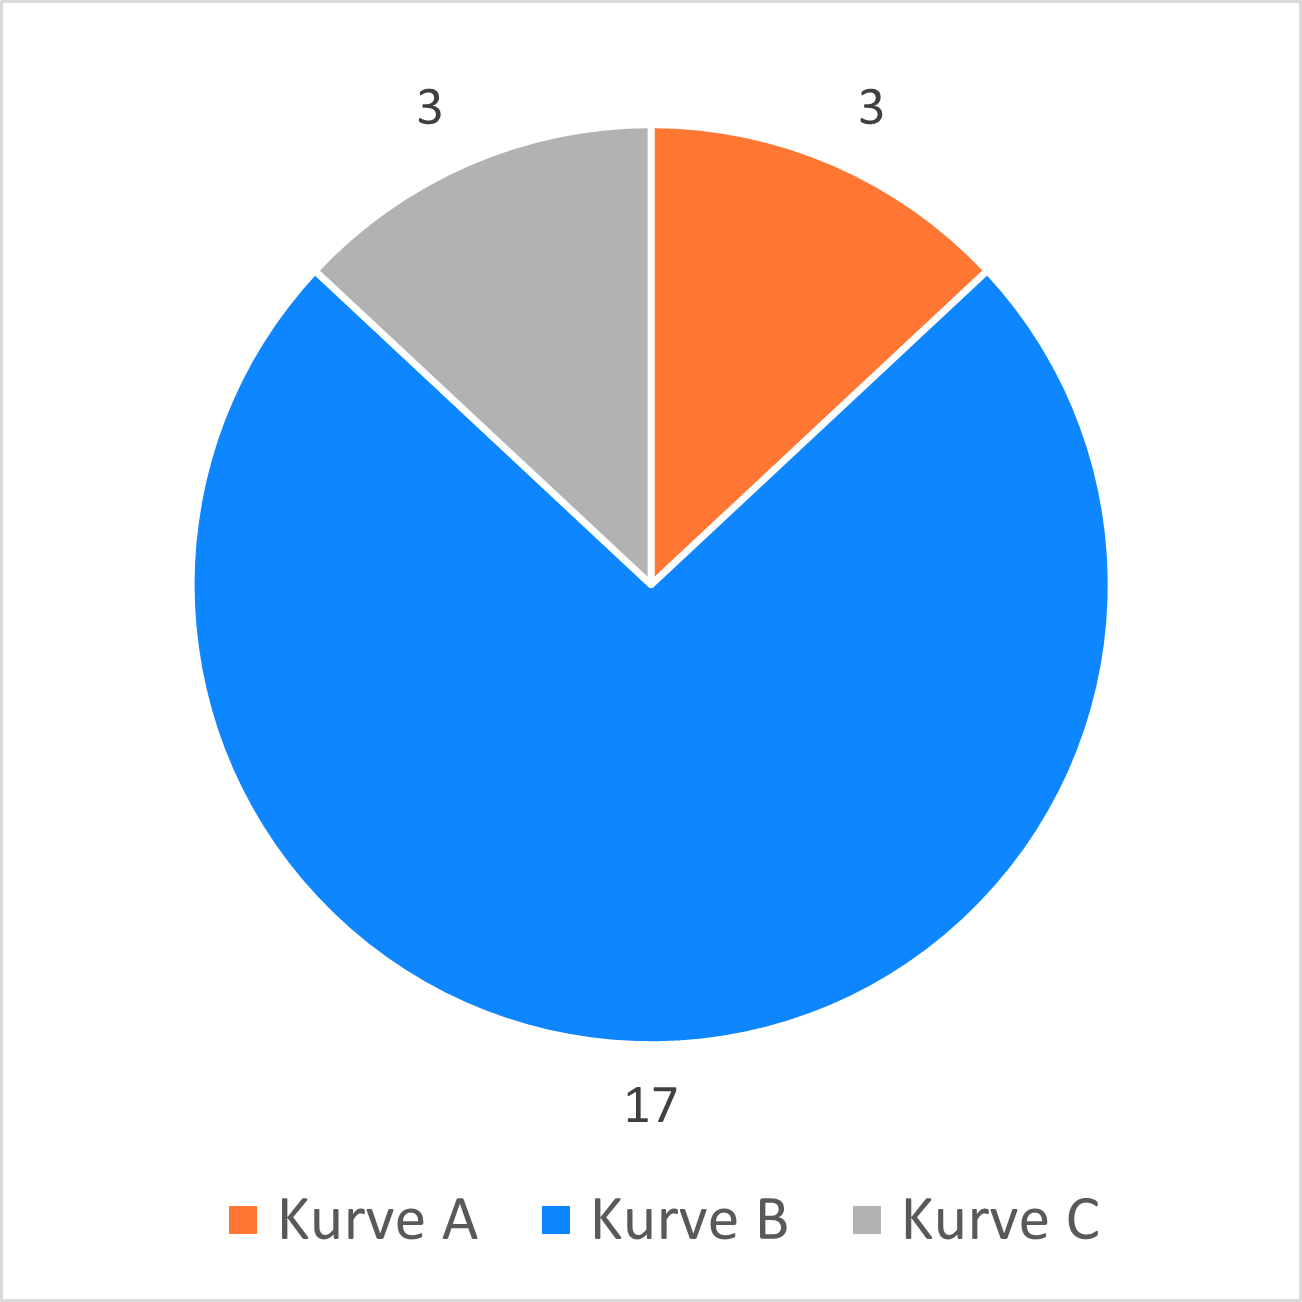
\includegraphics[width = 0.5\textwidth]{gfx/ergebis-kurve-mitarbeiter.png}}
	
	\caption{Umgang mit Unterforderung bei Projektmanagern und Mitarbeitern}
	\label{fig:ergebnisse:fallstudie:kurven:abb1}
\end{figure}

In Abbildung \ref{fig:ergebnisse:fallstudie:kurven:abb1} ist zu erkennen, dass sowohl die befragten Projektmanager als auch die teilnehmenden Mitarbeiter mehrheitlich angaben, Unterforderung bei der Projektarbeit vermeiden zu wollen.
\shorthandon{"}
